\chapter{Differentiation and Quadrature}

Numerous applications such as calculation of tangent vectors or areas lead to the problem of computing 
\begin{equation}
    \cD(f) := \frac{d}{dx} f(x),\quad \cI(f) := \int_a^b f(x) dx, 
\end{equation}
for certain function $f(x)\in C^k([a, b])$. The accurate evaluations would be sometimes difficult if the analytic expression is absent. Especially when the function values of $f$ are only accessible at a finite number of nodes. Therefore, it is important to find simple yet effective methods to approximate the derivatives and integrals. 


\section{Extrapolation}
From the previous discussion, we already know that interpolation is to provide an estimate \emph{within} the original observation range. The extrapolation is similar but aims to produce estimates outside the observation range. However, extrapolation may be subject to a greater uncertainty (Fig~\ref{FIG: EXTRAPO}), one should use it only when overestimate is hardly occurring.
\begin{figure}[!htb]
    \centering
    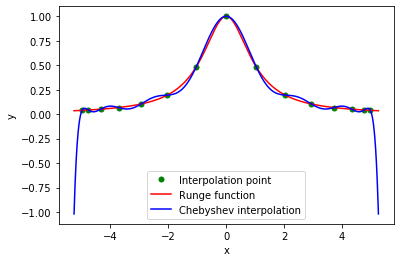
\includegraphics[scale=0.7]{extrapolate}
    \caption{Extrapolation behavior for Chebyshev interpolation with $15$ nodes.}
    \label{FIG: EXTRAPO}
\end{figure}

\subsection{Richardson Extrapolation}
Suppose there is a sequence of estimates $A(h)$ depending the parameter $h$, the limit $A^{\ast} = \lim_{h\to 0^{+}} A(h)$ is the quantity to be computed. In practice, we only have access to $A(h)$ for a few values of $h$. Using these values to estimate $A^{\ast}$ is a typical problem in extrapolation. 

The basic idea is to use polynomial interpolation with a sequence of nodes $h_j\to 0$. Suppose the function $A(h)$ admits the following asymptotic expansion:
\begin{equation}
    A(h) = a_0 + a_1 h^{\gamma} + a_2 h^{2\gamma} + \dots + a_k h^{k\gamma} + \cO(h^{(k+1)\gamma})
\end{equation}
for any $h > 0$ and $k\ge 0$. Then $A^{\ast} = a_0$ and $A(h) = A^{\ast} + \cO(h^{\gamma})$. Suppose we have access to the values $A(h_0),\dots, A(h_n)$, then this uniquely determines a polynomial $f_n\in\Pi_n$ and 
$f_n(h_j^{\gamma}) = A(h_j)$. We will approximate $A(0)\approx f_n(0)$. The computation of $f_n$ follows the construction of the Newton form. The error estimate 
\begin{lemma}
    Suppose $h_j$ can be represented as 
    $$h_j = \frac{\hbar}{t_j}$$
    for some adjustable $\hbar$ and scaling constants $ 1 < t_0 < t_1<\dots < t_{n-1}$. Then 
    $$f_n(0) = A^{\ast} + (-1)^n \frac{a_{n+1}}{\prod_{j=0}^n t_j^{\gamma}} \hbar^{(n+1)\gamma} + \cO(\hbar^{(n+2)\gamma}),\quad \text{as }\hbar\to 0.$$
\end{lemma} 
\begin{proof}
    We view $A(h)$ as a polynomial with respect to $h^{\gamma}$ of degree $(n+1)$ with an addition perturbation $\cO(h^{(n+2)\gamma})$. Then we have 
    \begin{equation}
        A(h) = p_{n+1}(h^{\gamma}) + \cO(h^{(n+2)\gamma}).
    \end{equation}
    Let $\tilde{f}_n$ be the interpolation polynomial of degree $n$ to $p_{n+1}$, 
    \begin{equation}
        p_{n+1}(x) \equiv \tilde{f}_n(x) + p[x, x_0, x_1, \dots, x_n] \prod_{j=0}(x - h_j^{\gamma}). 
    \end{equation}
    where $p[x, x_0, x_1, \dots, x_n]$ is the coefficient of $p_{n+1}$'s leading power, $a_{n+1}$. Thus 
    \begin{equation}
        A^{\ast} = p_{n+1}(0) = \tilde{f}_n(0) +a_{n+1} \prod_{j=0}(0 - h_j^{\gamma}). 
    \end{equation} 
    Use the result we have discussed in the stability of polynomial interpolation, see Chapter~\ref{SSec: 2-Sta-Pol-Int}. Therefore 
    \begin{equation}
        |\tilde{f}_n(0) - f_n(0)|\le \lambda_n(0) \cdot \cO(\hbar^{(n+2)\gamma})
    \end{equation}
    Here the Lebesgue function at zero $\lambda_n(0)$ is 
    \begin{equation}
        \lambda_n(0) = \sum_{j=0}^n \prod_{k=0, k\neq j}^n \left|\frac{h_k^{\gamma}}{h_k^{\gamma} - h_j^{\gamma}}\right| =  \sum_{j=0}^n \prod_{k=0, k\neq j}^n \left|\frac{1}{1 - (\frac{t_k}{t_j})^{\gamma}}\right|,
    \end{equation}
    which is independent of $\hbar$.
\end{proof}
The {Richardson extrapolation} considers the special choice of $t_j = t^j$ for some $t > 1$. The error estimate then is 
\begin{equation}
    f_n(0) = A^{\ast} + \left(\frac{(-1)^n}{t^{n(n+1)\gamma/2}} a_{n+1}\right) \hbar^{(n+1)\gamma} + \cO(\hbar^{(n+2)\gamma}).
\end{equation}
In fact, there are easier ways to calculate the Richardson extrapolation. Consider the following
\begin{equation}
    A(h) - t^{\gamma} A\left(\frac{h}{t}\right) = (1 - t^{\gamma}) A^{\ast} + \cancel{a_1 \left(h^{\gamma} - t^{\gamma} \left(\frac{h}{t}\right)^{\gamma}\right)} + a_2\left(h^{2\gamma} - t^{\gamma}\left(\frac{h}{t}\right)^{2\gamma}\right) +\dots
\end{equation}
Let $A_1(h) = \frac{A(h) - t^{\gamma} A(\frac{h}{t}) }{1 - t^{\gamma}} $, we obtain the first iteration result as 
\begin{equation}
    A^{\ast} \approx A_1(h) + \cO(h^{2\gamma}),
\end{equation}
then follow the same idea, we cancel the $\cO(h^{2\gamma})$ term by
\begin{equation}
    A_1(h) - t^{2\gamma} A_1\left(\frac{h}{t^2}\right) = (1 - t^{2\gamma}) A^{\ast} + \cO(h^{3\gamma}).
\end{equation}
Therefore by taking $A_2(h) = \frac{A_1(h)- t^{2\gamma} A_1(\frac{h}{t^{2\gamma}})}{1 - t^{2\gamma}}$, the second iteration satisfies 
\begin{equation}
    A^{\ast}\approx A_2(h) + \cO(h^{3\gamma}).
\end{equation}
However, it is not guaranteed that such process can constantly refine the approximation due to the potentially fast growing constant in the $\cO$ notation.

\subsection{Wynn's epsilon method}
The Wynn's $\eps$-method is another kind of extrapolation algorithm which is recommended as the best all-purpose acceleration method. It has a strong connection with Pad\'e approximation and continued fractions. We will not cover the detailed derivation of the theory behind in this section. However, the Wynn's $\eps$-method still has its limitation if the sequence converges to the desired value too slowly. The algorithm is stated as follows. Let $s_0, s_1, \dots, s_n,\dots$ be a sequence converging to the desired quantity,
\begin{enumerate}
    \item Initialization. For $j = 0, 1, 2,\dots$, set 
    $$\eps_{-1}^{(j)} = 0 \text{ (guarding elements)}, \quad \eps_{0}^{(j)} = s_j.$$
    \item Iteration. For $j,k = 0,1,2,\dots$, 
    $$\eps_{k+1}^{(j)} = \eps_{k-1}^{(j+1)} + [\eps_{k}^{(j+1)} - \eps_{k}^{j}]^{-1}.$$
\end{enumerate}
The extrapolated results are stored at the columns $\eps_{2l}^{(j)}$, $j, l=0,1, \dots$.
\begin{example}
    It is known that $\pi/4$ can be calculated by the asymptotic expansion:
    \begin{equation}
        \arctan z = z - \frac{z^3}{3} + \frac{z^5}{5} - \dots 
    \end{equation}
    at $z = 1$. Define the function $A(h)$ such that 
    \begin{equation}
        A(h)= \sum_{j=0}^{1/h} \frac{(-1)^j}{2 j + 1} = \frac{\pi}{4} + a_1 h + a_3 h^3 + \dots
    \end{equation}
    Then we can approximation error is $\cO(h)$, which is very slow. Taking $h=10^{-3}$ has around $2\times 10^{-4}$ error. 
    \begin{enumerate}
        \item     With Richardson Extrapolation, we can take $1/h = 250, 500, 1000, 2000$ and calculate the Richardson extrapolation three times would result with almost machine accuracy.
        \item With Wynn's $\eps$-method, we may take the sequence 
        $$s_k = \sum_{j=0}^k \frac{(-1)^j}{2 j + 1}$$
        as the truncated series at $z = 1$. With about 20 terms, we already reach the machine accuracy.
    \end{enumerate}

\end{example}
\section{Differentiation with Finite Difference}
Let $f\in C^2([a, b])$, we recall the Taylor expansion with reminder term, 
\begin{equation}
    f(x + h) = f(x) + h f'(x) + \frac{h^2}{2} f''(\xi),
\end{equation}
where $\xi = \xi(x)\in [a, b]$, therefore we can compute the derivative by 
\begin{equation}
    f'(x)  = \frac{f(x + h) - f(x)}{h} - \frac{h}{2} f''(\xi).
\end{equation}
This approximation offers a way to evaluate the derivative $f'(x)$ with error term $\cO(h)$. Also the above formula is \emph{exact} when $f$ is polynomial of degree $1$. We say an approximation has ``degree $k$ accuracy'' if the approximation is \emph{exact} for any polynomial of degree $k$. 

Another important terminology is the ``order''. It describes the error term of the approximation. In the above case, the error term scales like $\cO(h)$ as $h\to 0$, then the approximation is ``of order $1$'' or ``first order''. In general, if the error term behaves like $\cO(h^p)$, then we can say it is $p$-th order approximation. 

The ``stencil'' refers to a set of nodes used in the approximation. In the above example, we have used $x, x+h$. We can of course create its sibling
\begin{equation}
    f'(x) = \frac{f(x) - f(x - h)}{h} + \frac{h}{2} f''(\zeta),
\end{equation}
which uses the nodes $x-h, x$. When all nodes are $\ge x$ or $\le x$, we say the scheme is forward or backward, respectively.

\subsection{Finite Difference from Taylor Expansion}
All results related to finite difference can be easily derived from Taylor expansion. Suppose we would like to approximate a high order derivative $f^{(m)}(x)$ with some nodes scattered around $x$ in the following form. 
\begin{equation}
    \frac{1}{h^m} \sum_{j = 0}^n c_j f(x + a_j h) = f^{(m)}(x) + E(x, h)
\end{equation}
where $E$ is the error term and $a_j\in\bbZ$ (sometimes half integers are used). Since $h\to 0$, we can expand all $f(x + a_j h)$ locally by Taylor series and truncate at least order $(m+1)$.
\begin{equation}
    \frac{1}{h^m} \sum_{j=0}^n c_j \left( \sum_{k=0}^{p} \frac{1}{p!}f^{(p)}(x) a_j^p h^p + \frac{f^{(p+1)}(\xi_j)}{(p+1)!} a_j^{p+1} h^{p+1}\right)
\end{equation} 
Clearly, we need all lower (and maybe higher than $m$-th) order derivatives of $f$ cancelled in the above summation, which is 
\begin{equation}
    \begin{aligned}
        \sum_{j=0}^n c_j a_j^p &= 0,\quad 0\le p < m,    \\
        \sum_{j=0}^n c_j a_j^m &= {m!}, \\
    \end{aligned}
\end{equation}
It is straightforward that $n \ge m$, otherwise the first equation system (Vandermonde matrix) must have zero solution.  Suppose we have found a solution $(c_j, a_j)$, $j=0,\dots, n$,  to the above system, then in the sequel, we try to estimate the error term $E(x, h)$. Especially, if $n = m$, here are two cases, let the following constant $C$ 
$$       C =  \sum_{j=0}^n c_j a_j^{m+1}, \quad \text{$C$ could be zero}. $$
\begin{enumerate}
    \item If $C = 0$, then the error term can be estimated by expanding to $(m+2)$-th derivative. 
    \begin{equation}\label{EQ: ERROR FD}
        E(x, h) = \frac{1}{h^m}\sum_{j=0}^n c_j \frac{f^{(m+2)}(\xi_j)}{(m+2)!} a_j^{m+2} h^{m+2} = h^2 \left(\sum_{j=0}^n c_j  a_j^{m+2}\frac{f^{(m+2)}(\xi_j)}{(m+2)!}\right)\,.
    \end{equation}
    One can expect higher order accuracy when more terms are involved. 
    \item If $C\neq 0$, then the error term is 
    \begin{equation}\label{EQ: ERROR FD NZERO}
        E(x, h) = \frac{1}{h^m}\sum_{j=0}^n c_j \frac{f^{(m+1)}(\xi_j)}{(m+1)!} a_j^{m+1} h^{m+1} = h \left(\sum_{j=0}^n c_j  a_j^{m+1}\frac{f^{(m+1)}(\xi_j)}{(m+1)!}\right)\,.
    \end{equation}
\end{enumerate}
\begin{remark}
    Here the $\xi_j$, $j=0,\dots,n$ are in general distinct but possible to choose a single $\xi$ to simplify the representation through the intermediate value theorem. 
\end{remark}
\begin{lemma}\label{LEM: FD COEF}
    If $f\in C^{m+1}(\cI)$, where $\xi_j\in\cI$, then there exists $\xi\in \cI$ such that 
    \begin{equation}
        \sum_{j=0}^n c_j  a_j^{m+1}\frac{f^{(m+1)}(\xi_j)}{(m+1)!} =   \sum_{j=0}^n c_j  a_j^{m+1}\frac{f^{(m+1)}(\xi)}{(m+1)!},
    \end{equation}
    if $c_j a_j^{m+1}\ge 0$ (or $\le 0$), $j=0,\dots, n$. 
\end{lemma}
\begin{proof}
    Define $$\psi(x) =  \sum_{j=0}^n c_j  a_j^{m+1}\frac{f^{(m+1)}(x) - f^{(m+1)}(\xi_j)}{(m+1)!}$$
    then $\max_j f(\xi_j)\ge 0$ and $\min_j f(\xi_j) \le 0$. Then apply the intermediate value theorem. 
\end{proof}

\begin{example}
    Let $n = 2, m = 2$ for an example. Then the equation system becomes 
    \begin{equation}\label{EQ: EXAM FD}
        \begin{aligned}
            c_0  + c_1  + c_2  &= 0, \\
            c_0 a_0 + c_1 a_1 + c_2 a_2 &= 0, \\
            c_0 a_0^2 + c_1 a_1^2 + c_2 a_2^2 &= 2.  
        \end{aligned}
    \end{equation}
    Then using Gauss elimination, one can find that 
    $$c_2 (a_2 - a_0) (a_2 - a_1) = 2.$$
    The above formula can be generalized. The constant $C = c_2(a_2 - a_0)(a_2 - a_1) (a_0 + a_1 + a_2)$. We list a few possible choices to satisfy~\eqref{EQ: EXAM FD}. 
    \begin{enumerate}
        \item $(a_0, a_1, a_2) = (-1, 0, 1)$, $c_2 = 1$. Then $c_0 = 1$ and $c_1 = -2$ are derived. In this case $C = 0$. We will have the error term 
        $$E(x, h) = \frac{h^2}{24}\left(f^{(4)}(\xi_0) + f^{(4)}(\xi_2)\right) \underbrace{\Longrightarrow }_{\ref{LEM: FD COEF}} \frac{h^2}{12} f^{(4)}(\xi).$$
        This is called central difference scheme.
        \item $(a_0, a_1, a_2) = (0, 1, 2)$, $c_2 = 1$. Then $c_1 = -2$, $c_0 = 1$,  $C \neq 0$. The error is 
        $$E(x, h) = \frac{h}{6} (f^{(4)}(\xi_1) + 8 f^{(4)}(\xi_2)) \underbrace{\Longrightarrow }_{\ref{LEM: FD COEF}} \frac{3h}{2} f^{(4)}(\xi).$$
        This is the forward difference scheme.
    \end{enumerate}
    The combination of the coefficients is not unique. The central scheme has better approximation due to its symmetry. In fact any combination satisfying $a_0 + a_1 + a_2 = 0$ should have the same order of error.
\end{example}
The general scheme with $a_j = j$ (or $-j$) can be derived from the following theorem.
\begin{theorem}\label{THM: FWD DIFF}
    In general, if $n = m$, then the forward difference scheme satisfies 
    \begin{equation}
        \begin{aligned}
            \sum_{j=0}^n (-1)^{n-j} \binom{n}{i} j^p &= 0,\quad 0\le p < n \\
            \sum_{j=0}^n (-1)^{n-j} \binom{n}{i} j^n &= n!.   
        \end{aligned}
    \end{equation}
\end{theorem}
\begin{proof}
    It is the easiest to prove by binomial transform. It can be also proved through the induction easily. Let 
    $$P_0(x) = (x - 1)^n,\quad P_k(x) =  x P'_{k-1}(x) ,$$
    then one can show inductively that $P_k$, $k\ge 1$, has following form
    \begin{equation}\label{EQ: BINOM}
        P_k(x) = n(n-1)\cdots (n-k+1) (x - 1)^{n-k} x^k  + (x-1)^{n-k+1} F(x)
    \end{equation}
    with $F(x)$ as a polynomial of at most degree $k-1$. This can be easily proved since 
    \begin{equation}
        \begin{aligned}
           P_{k+1} =  x P_k'(x) &= n(n-1)\cdots (n-k)(x-1)^{n-k-1} x^{k+1} + \\&\quad +   (x-1)^{n-k} { n(n-1)\cdots (n-k+1) k x^k}  \\
           &\quad + (x-1)^{n-k} {(n-k+1)  F(x)}\\
           &\quad+(x-1)^{n-k} {(x-1)F'(x)}.
        \end{aligned}
    \end{equation}
    It is clear the last three terms can merge into the form as~\eqref{EQ: BINOM}. Therefore $P_k(1) = 0$ unless $k = n$ and $P_n(1) = n!$ is immediately obtained. 

    Now if we expand the polynomial $P_0$ as monomial, 
    \begin{equation}
        P_0(x)=\sum_{j=0}^n \binom{n}{j} x^j (-1)^{n-j}, 
    \end{equation}
    then it is not difficult to show that 
    $$P_k(x) = \sum_{j=0}^n \binom{n}{j} j^k x^j (-1)^{n-j}$$
    through induction as well, which is exactly our conclusion by setting $x = 1$.
\end{proof}
\begin{theorem}[forward difference]\label{THM: FORWARD FD}
    $$f^{(n)}(x) = \frac{1}{h^n}\sum_{j=0}^n (-1)^{n-j} \binom{n}{j} f(x + j h) + \cO(h).$$
    The corresponding schemes of backward difference and central difference can be derived similarly (see the exercise).
\end{theorem}
\subsection{Rounding Error Issue}
The finite difference formula provides a simple and effective way to evaluate the derivatives, however its formulation would be sensitive to rounding errors. Take the central difference scheme for $f''(x)$ as an example, one can derive a similar estimate for higher order derivatives.
\begin{example}
    \begin{equation}
        f''(x) = \frac{f(x + h) - 2 f(x) + f(x - h)}{h^2} + \frac{h^2}{12}f^{(4)} (\xi)
    \end{equation}
    The error comes from two sources. The truncation error term from $\frac{h^2}{12} f^{(4)}(\xi)$ and the rounding error from the evaluation of the first term by the basic arithmetic operations.  Suppose the addition/subtraction are implemented by Kahan sum (see exercises of Chapter 1) which almost does not introduce errors in the arithmetic operations. Then the rounding error of $f(x + h) - 2 f(x) + f(x - h)$ is at most $4 \max_{x\in \cI} |f(x) | \textup{u}$.  Therefore the total error
    \begin{equation}\label{EQ: RD ERR}
        |E_{total}|\le \frac{4 \max_{x\in \cI} |f(x) | \textup{u}}{h^2} + \frac{h^2}{12} \max_{x\in \cI} |f^{(4)} (x)|
    \end{equation}
    Minimizing the right-hand-side of~\eqref{EQ: RD ERR}, let $M = \max_{x\in\cI} |f(x)| \max_{x\in\cI} |f^{(4)}(x)|$, we obtain 
    $$\min_{h\in\bbR} |E_{total}| \le \sqrt{\frac{4}{3}\textup{u} M }.$$
    The optimal achieves at $h^{\ast} = \sqrt[4]{48\textup{u}M}$. For example, if $f(x) = \exp(x)$ and evaluate its second derivative around $x = 0$, then $\cM\sim 1$, the error is around $1.3\times 10^{-8}$ for $h^{\ast}\sim 2.5\times 10^{-4}$. 
\end{example}
For higher order derivatives, the rounding error would have even greater impact for the finite difference schemes. Then it is much more important to avoid $h$ being too small. 
\subsection{Improve by Extrapolation}
Now we can combine the previous discussed extrapolation technique to acquire higher ordered scheme. We use a very simple example to show how this works. 
\begin{example}
    Suppose $A(f, h)$ is the central difference scheme for $f'(x)$, which is 
    \begin{equation}
        A(f, h) = \frac{f(x + h) - f(x- h)}{2h}
    \end{equation}
    the previous discussion has claimed that $A(f, h) = f'(x) + \cO(h^2)$. Now we try to fit the formulation in the framework of extrapolation. Formally, we can expand $f(x\pm h)$ with Taylor series with infinite terms (might not converge though), that is, 
    \begin{equation}
        \begin{aligned}
            f(x + h) &= f(x) + h f'(x) + \frac{h^2}{2} f''(x) + \frac{h^3}{6} f'''(x) + \cdots \\
            f(x - h) &= f(x) - h f'(x) + \frac{h^2}{2} f''(x) - \frac{h^3}{6} f'''(x) + \cdots 
        \end{aligned}
    \end{equation}
    Therefore $A(f, h) = f'(x) + \frac{h^2}{6} f''(x) + \frac{h^4}{120}f''''(x) + \cdots $. Here the coefficients are all formal since the convergence is not guaranteed. In the next, we take $A(f, \frac{h}{2})$, which uses a smaller step length to approximate $f'(x)$, then 
    \begin{equation}
        A(f, h/2) =  f'(x) + \frac{h^2}{24} f''(x) + \frac{h^4}{1920}f''''(x) + \cdots
    \end{equation}
    Cancel the $\cO(h^2)$ term by $$\frac{1}{3}\left( 4 A(f, h/2) - A(f, h) \right) =  f'(x) - \frac{h^4}{480} f''''(x) +\cdots. $$
    In this way we have built a more accurate  formula $A_1(f, h) = \frac{4 A(f, h/2) - A(f, h)}{3}$ for $f'(x)$, the error is fourth order. Bring the definition of the finite difference scheme into $A_1$, then 
    \begin{equation}
        \begin{aligned}
        A_1(f, h) &= \frac{4}{3} \left(\frac{f(x + h/2) - f(x - h/2)}{h}\right) - \frac{1}{3} \left(\frac{f(x + h) - f(x - h)}{2h}\right) \\
        &= \frac{-f(x+ h) + 8 f(x + h/2) - 8 f(x - h/2) + f(x - h)}{6h}.
        \end{aligned}
    \end{equation}
    This central difference scheme has $\cO(h^4)$ error. 
\end{example}
The above example can still iterate through the extrapolation process, since $A_1(f, h) = f'(x) + \cO(h^4)$, we can use $A_2(f, h) = \frac{16}{15}A_1(f, h/2) -  \frac{1}{15}A_1(f, h)$ to cancel out the $\cO(h^4)$ term which leads to a $\cO(h^6)$ error. However one should also notice this process require more nodes for computation: $A_1$ needs nodes $x\pm h$, $x\pm h/2$, $A_2$ will acquire additional nodes $x\pm h/4$ for evaluation. Such higher precision evaluation method takes more computational time, sometimes we need to trade off the efficiency and accuracy.

\begin{remark}
    One of the advantage of using extrapolation is that $h$ does not have to be too small which is sensitive to numerical rounding errors. The potential issue would be growth of derivative with respect to order, for sufficiently smooth functions, extrapolation usually produces quite accurate evaluations. The potential limitation of the Richardson extrapolation is the requirement of known asymptotic expansion (formally only), while the Wynn-$\eps$ method does not have such limitation. 
\end{remark}


\section{Quadrature Rules}
The numerical quadrature find the value of an integral 
$$\cI(f) = \int_a^b f(x) dx $$
from the function values at a finite number of points. We are mostly interested in the following quadrature formula 
\begin{equation}
    \cI_n(f) = (b - a) \sum_{j=0}^n w_j f(x_j)
\end{equation}
where $x_j$ are the nodes and $w_j$ are the weights. Similar to the numerical derivatives, we also define some terminologies. The formula $\cI_n$ is said to have degree $k$ accuracy if $\cI_n$ is exact for all polynomials $f\in\Pi_k$. Since the integration formula is linear, the exactness can be rephrased as 
\begin{equation}
    \begin{aligned}
        \cI(x^p) &= \cI_n(x^p),\quad 0\le p \le k, \\
        \cI(x^{k+1}) &\neq \cI_n(x^{k+1}) .   
    \end{aligned}
\end{equation}
\subsection{Interpolation Based Rules}
The interpolation based idea is intuitive. Let $q_n(x)$ be the interpolation polynomial on the nodes $x_j$ with values $f(x_j)$, $j=0,1,\dots, n$, respectively. We define the quadrature by interpolation formula as 
\begin{equation}
    \cI_n(f):= \int_a^b q_n(x) dx 
\end{equation}
The above quadrature formula is exact for all degree $n$ polynomials $f$, therefore it has \underline{at least} degree $n$ accuracy. 

\begin{remark}
    In the section of interpolation, we have seen that the $L^{\infty}$ error between $f$ and $q_n$ could be large (e.g. Runge phenomenon) as $n\to \infty$. So the nodes would be important as well for quadratures.
\end{remark}
Using the Lagrange polynomials, we can represent 
\begin{equation}
    q_n(x) = \sum_{j=0}^n f(x_j) L_j(x),\quad L_j(x) = \prod_{k=0, k\neq j}^n \frac{x - x_k}{x_j - x_k}. 
\end{equation}
Then it is not difficult to derive
\begin{equation}
    \begin{aligned}
        \cI_n(f)& = \sum_{j=0}^n f(x_j) \int_a^b L_j(x) dx  \\ &=(b-a) \sum_{j=0}^n f(x_j) \int_0^1 \prod_{k=0, k\neq j }^n \frac{t - t_k}{t_j - t_k} dt, \quad t_j = \frac{x_j - a}{b-a}.   
    \end{aligned}
\end{equation}
therefore the weights $w_j =  \int_0^1 \prod_{k=0, k\neq j }^n \frac{t - t_k}{t_j - t_k} dt$. 

\begin{example}[rectangle rule]
   The rectangle rule is the simplest one, where we choose $x_0 = \frac{a+b}{2}$ as the middle point. Then the quadrature rule writes
   $$\cI_{0, rectangle}(f)  = (b-a) f(x_0). $$
  Such rule is exact for any linear functions, therefore it has degree $1$ accuracy. We can see that the degree of exactness could exceed $n$. Later we will see the maximum degree of exactness for such form is $2n+1$ in the next chapter.
\end{example}

\begin{example}[trapezoid rule]
The trapezoid rule takes $x_0 = a$ and $x_1= b$. 
$$\cI_{1,trapezoid} (f) = (b-a)\left( \frac{1}{2} f(x_0) + \frac{1}{2} f(x_1) \right).$$
One can check that this rule is exact for $f(x) = 1, x$. It is also having degree $1$ accuracy. It actually has a slightly larger constant in error estimate than the rectangle rule.
\end{example}
\subsection{Numerical Error of Interpolation Based Rules}
Now we try to estimate $|\cI(f) - \cI_n(f)|$ from above derivation. 
\begin{theorem}\label{THM: ERROR QUAD RULE}Suppose the quadrature rule $\cI_n$ has at least degree $r$ accuracy that $r\ge n$ and $f\in C^{r+1}([a, b])$. 
    Then 
    \begin{equation}
        |\cI(f) - \cI_n(f)| \le \Omega_r \frac{(b-a)^{r+2}}{(r+1)!} \max_{x\in[a, b]} |f^{(r+1)}(x)|,
    \end{equation}
    where the constant $\Omega_k$ is defined by 
    \begin{equation}
        \Omega_r := \min_{t_{n+1}, \dots, t_r\in [0, 1]} \int_0^1 \prod_{j=0}^r |t - t_j| dt, \quad t_j = \frac{x_j - a}{b-a}, j=0,\dots, n.
    \end{equation}
\end{theorem}
\begin{proof}
    Let $x_{n+1}, \dots, x_{r}$ be additional distinct nodes on $[a, b]$ and define $f_r$ the interpolating polynomial on the nodes $x_0,\dots, x_r$, since the quadrature rule has degree $r$ accuracy, then 
    $$\cI_n(f) = (b-a)\sum_{j=0}^n w_j f(x_j) = (b-a)\sum_{j=0}^n w_j f_r(x_j) = \cI_n(f_r) = \cI(f_r).$$
    Using the theories developed in Interpolation, we know that 
\begin{equation}
    f(x) - f_r(x) = \frac{\omega_r(x) f^{(r+1)}(\xi)}{(r+1)!},
\end{equation}
where $\omega_r(x) = \prod_{j=0}^r (x - x_j)$, therefore 
\begin{equation}
   | \cI(f - f_r)| = \left| \int_a^b \frac{\omega_r(x) f^{(r+1)}(\xi)}{(r+1)!} dx \right|\le \frac{(b-a)}{(r+1)!} \left(\int_a^b |\omega_r(x)|dx \right)  \max_{x\in[a,b]}|f^{(r+1)}(x)|.
\end{equation}
Since $x_{n+1},\dots, x_r$ can be chosen arbitrarily, then we select the combination that minimizes $  \left(\int_a^b |\omega_r(x)|dx \right)$, which will lead to our conclusion by a simple scaling.
\end{proof}
\begin{remark}
    As we can see, the error from interpolation based quadrature has a similar form of the interpolation polynomial's error. This implies the Runge phenomenon would occur as well. In fact, the Runge function's integration will not converge on uniformly distributed nodes.
\end{remark}
One way to overcome the issue of Runge phenomenon is to perform piecewise integration. Suppose $[a, b]$ is divided into $N$ sub-intervals of equal sizes, each has length $H = \frac{b-a}{N}$. Then the quadrature error on each sub-interval would be:
$$\Omega_r \frac{H^{r+2}}{(r+1)!}   \max_{x\in[a,b]}|f^{(r+1)}(x)|$$
where $\Omega_r$ is independent of the interval length. Therefore the total quadrature error would be bounded by 
$$N\Omega_r \frac{H^{r+2}}{(r+1)!}   \max_{x\in[a,b]}|f^{(r+1)}(x)| =  (b-a)\Omega_r \frac{H^{r+1}}{(r+1)!}   \max_{x\in[a,b]}|f^{(r+1)}(x)| =\cO((b-a)H^{r+1}).$$
\begin{example}[rectangle rule] 
    For rectangle rule, $r = 1, n= 0$, therefore 
    \begin{equation}
        \Omega_r = \min_{t_1} \int_0^1 |t - \frac{1}{2}||t - t_1| dt  = \frac{1}{12}, \quad (t_1 = \frac{1}{2}).
    \end{equation}
This is easiest to notice by changing variable $s = t - \frac{1}{2}$ and the symmetry, then the integral is just 
$$\Omega_r = \min_{z\in [-1/2, 1/2]} \int_{-1/2}^{1/2} |s||s - z| ds =  \min_{z\in [0, 1/2]} \int_{0}^{1/2} s (|s - z| + |s + z|) ds \ge   \int_{0}^{1/2} s (2s) ds. $$ 
\end{example}
\begin{example}[trapezoid rule]
    For trapezoid rule, $r = n = 1$, therefore 
    \begin{equation}
        \Omega_r = \int_0^1 (1-t)t dt = \frac{1}{6}.
    \end{equation}
    then the error is bounded by $\frac{(b-a)h^2}{12}  \max_{x\in[a,b]}|f^{(r+1)}(x)|$. 
\end{example}

\subsection{Newton-Cotes Formula}
The Newton-Cotes formula is a special interpolation based quadrature rule. The nodes are \underline{equally spaced}. The rectangle and trapezoid rules are just two simplest cases. We define 
\begin{enumerate}
    \item closed form, $x_0 = a$, $x_n = b$, $x_j = a  + jh$, $h = \frac{b-a}{h}$, $n\ge 1$. 
    \item open form, $x_0 = a + h$, $x_n = b - h$, $h = \frac{b-a}{n+2}$, $n\ge 0$.
\end{enumerate}
The difference is whether the end points are included or not. Using the previous result, we can compute the quadrature weights by 
\begin{equation}
    \begin{aligned}
        w_j &= \int_0^1 \prod_{k=0, k\neq j}^n \frac{t - t_k}{t_j - t_k} dt =  \int_0^1 \prod_{k=0, k\neq j}^n \frac{nt - k}{j- k} dt \\
        &=\frac{1}{n}\int_0^n \prod_{k=0, k\neq j}^n \frac{s - k}{j - k} ds. 
    \end{aligned}
\end{equation}
The computations of the weights can be efficient by noticing the symmetry. 
\begin{lemma} $w_j = w_{n - j}.$
\end{lemma}
\begin{proof}
    This is because $w_j = \int_a^b L_j(x) dx = \int_a^b L_j(a + b - x) dx = \int_a^b L_{n-j}(x) dx = w_{n-j}.$
\end{proof}

The weights $w_j$ are only relevant to $n$ and $j$. In practice, these values are tabulated \emph{a priori}. When $n\ge 2$, the weights include negative terms for \underline{open forms}, and when $n\ge 8$, the weights include negative terms for \underline{closed forms}, which could introduce numerical instability from rounding errors. Therefore one should only limit to small values of $n$.
\begin{remark}
    We can derive the error estimate for Newton-Cotes formula using the result from last section. 
    \begin{equation}
        \begin{aligned}
            |\cI(f) - \cI_{n,NC}(f)| &\le \Omega_r \frac{(b-a)^{r+2}}{(r+1)!}\\
&= M_n  h^{r+2} \max_{x\in[a, b]} |f^{(r+1)}(x)| 
    \end{aligned}
    \end{equation}
    where $M_n = \Omega_r n^{r+2}\frac{1}{(r+1)!}$, see the following table for a reference.
\end{remark}
\begin{table}[!htb]
    \caption{A few examples for closed form}
    \vspace{0.2cm}
    \centering
        \begin{tabular}{ c| l c  c}
            \hline 
            $n$ & $w_j$ & $r$ & $M_n$ \\ 
            \hline 
            \hline 
            1 & ($1/2$, $1/2$) & $1$ & $1/12$\\  
            2 &  ($1/6$, $2/3$, $1/6$)  & $3$ & $1/90$ \\
            3 & ($1/8$, $3/8$, $3/8$, $1/8$)& $3$ & $3/80$\\
            4 & ($7/90$, $32/90$, $12/90$, $32/90$, $7/90$) & $5$ & $8/945$\\
            \hline
           \end{tabular}
    \end{table}
    From the above table, we can notice that when $n$ is even, the exactness is at $r = n+1$ for closed forms. This actually is a general statement. 
\begin{lemma}
    For $n\ge 2$ even, the closed forms of Newton-Cotes formula have degree $r = n+1$ accuracy.
\end{lemma}
\begin{proof}
    First, we know that $r\ge n$. Consider any polynomial of degree $n+1$, 
    \begin{equation}
        p(x) = \sum_{j=0}^{n+1} b_j x^j, 
    \end{equation}
    we can rewrite the polynomial by 
    \begin{equation}
        p(x) = b_{n+1} (x - \frac{a+b}{2})^{n+1} + \sum_{j=0}^n b'_j x^j 
    \end{equation}
    with another set of coefficients $b_j'$. The first term will have the integral as zero on the interval $[a, b]$. Numerically, using Newton-Cotes formula, 
    \begin{equation}
        \cI_{n, NC}( (x - \frac{a+b}{2})^{n+1}  ) = (b-a)\sum_{j=0}^n w_j  (x_j - \frac{a+b}{2})^{n+1}
    \end{equation}
    while $x_{n-j} -  \frac{a+b}{2} = -(x_j -  \frac{a+b}{2}) $ and $w_j = w_{n-j}$, we can cancel all terms. 

    It still remains to show that $\cI(x^{n+2})\neq \cI_{n,NC}(x^{n+2})$. Because $r= (n+1)$ degree of accuracy is achievable, then we borrow the previous estimate result, let $f(x) = x^{n+2}$, 
    \begin{equation}
        \begin{aligned}
            \cI(f) - \cI_n(f) &= \int_a^b \frac{\omega_{n+1}(x) f^{(n+2)}(\xi)}{(n+2)!} dx = \int_a^b \omega_{n+1}(x) dx \\
            &=     \int_a^b \omega_n(x) (x - x_{n+1}) dx = F(x) (x - x_{n+1})|_a^b - \int_a^b F(x) dx  
        \end{aligned}
    \end{equation}
    where $F(x)$ is defined by 
    $$F(x) := \int_a^x \omega_{n}(t) dt. $$ Then it is simple to derive that $F(a) = F(b) = 0$ using the symmetry. Now we only have to show that 
    $$\int_a^b F(x)dx \neq 0.$$
    In fact, we can show a stronger claim: $F(x)>  0$ over $(a, b)$. This is left as an exercise.
\end{proof}
Since the Newton-Cotes formula definitely will fail on evaluating the integral of Runge function $f(x) = \frac{1}{1+x^2}$ on the interval $[-5,5]$. It is more practical to combine the piecewise integral technique, which is called composite Newton-Cotes formula. In the following, we discretize the interval $[a, b]$ into $m$ sub-intervals of the same size $H = \frac{b-a}{m}$, then on each sub-interval, we apply the Newton-Cotes formula (say closed form) with $(n+1)$ equally spaced nodes. Then the numerical integral would have an error bounded by 
\begin{equation}
    m M_n \left(\frac{H}{n}\right)^{r+2} \max_{x\in[a, b]}|f^{(r+1)}(x)| =     (b-a) \frac{M_n}{n} \left(\frac{H}{n}\right)^{r+1} \max_{x\in[a, b]}|f^{(r+1)}(x)|
\end{equation}
where $r = n$ for odd $n$ and $r = n+1$ for even $n$, see last section for a quick derivation.

\begin{example}[composite trapezoid rule]
    The composite trapezoid rule is often used for practical integration especially when $f$ is periodic. Let $x_j = a + j H$, $j=0,\dots, m$, 
    $$T(f, H) = \frac{H}{2} \left(   f(a) + 2\sum_{j=1}^{m-1} f(x_j)  + f(b)  \right).$$
    Its error then can be estimated by
    \begin{equation}
        \frac{1}{12} (b-a) H^{2} \max_{x\in[a,b]} |f''(x)| =\cO((b-a)H^2).
    \end{equation}

\end{example}
In the next, we take a more careful look at the composite trapezoid rule. Recall the asymptotic Euler-Maclaurin summation formula: 
\begin{equation}
\sum_{j=0}^m g(j) \sim \int_0^m g(x) dx + \frac{g(0) + g(m)}{2} + \sum_{k=1}^{\infty} \frac{B_{2k}}{(2k)!}(g^{{2k-1}}(m) - g^{(2k-1)}(0))
\end{equation}
If we take $g(j) = f(a + jH)$, then we will arrive at 
\begin{equation}
    T(f, H)\sim \int_a^b f(x) dx + \sum_{k=1}^{\infty} \frac{B_{2k}}{(2k)!} H^{2k}\left(f^{(2k-1)}(b) - f^{(2k-1)}(a) \right) 
\end{equation}
which means there is an asymptotic expansion in the form of 
\begin{equation}\label{EQ: TRAP EXP}
    T(f, h) = \int_a^b f(x) dx + c_2 H^2 + c_4 H^4 + \cdots.
\end{equation}
Particularly, for smooth periodic function, the Euler-Maclaurin summation \emph{formally} shows the numerical error is less than any polynomial of $H$.
\subsection{Romberg Integration}
The composite trapezoid rule's asymptotic expansion~\eqref{EQ: TRAP EXP} implies a Richardson extrapolation combination to accelerate the evaluation. The Romberg integration refers to the following scheme: 
\begin{enumerate}
    \item Compute the sequence $a_{l, 0} = T(f, (b-a)/2^l)$, $l=0,\dots, L$, for the standard composite trapezoid rule with different sub-interval sizes. 
    \item Extrapolation by 
    $$a_{l, q+1} = \frac{4^{q+1} a_{l, q} - a_{l-1, q}}{4^{q+1} - 1}, \quad q = 0,\dots, L-1 \text{ and } l = q+1,\dots, L$$
    \item Output $a_{L,L}$, which should have an error of $\cO(H^{2L+2})$, $H = (b-a)/2^L$.
\end{enumerate}
\begin{remark}
    One of advantage of the Romberg method is the re-use of the nodes. This is extremely helpful when evaluating $f$ is not cheap. The extrapolation process also builds a new quadrature formulation implicitly. This quadrature rule brings the error $\cO(n^{-2})$ to $\cO(n^{-2\log_2 n-2})$, where $n$ is the total number of nodes. Although the computational time increases a few times, the return seems worth it when $f$ is sufficiently smooth.
\end{remark}
% \subsection{Gauss Quadrature}
% \subsection{Quadrature of Periodic Function}
\subsection{Adaptive Integrations}
Numerically, we can apply any composite quadrature rule on a successive partition of $[a, b]$ until the estimated error is under tolerance. Let $A(f, H)$ denote any composite quadrature rule (e.g. Newton-Cotes), $H = (b-a)/m$, then 
\begin{equation}
    A(f, H) = \int_a^b f(x) dx + \cO(H^{r+1})
\end{equation}
where $r$ is the degree of accuracy. Then $A(f, H/2)$ will presumably introduce an error of about $2^{-(r+1)}$ times the size of the previous case. Therefore we obtain an rough estimate of the error by 
$$\cE \approx \left|\frac{A(f, H) - A(f, H/2)}{1 - 2^{-(r+1)}}\right|$$
One can successively halve $H$ until the estimated error is less than tolerance. However such method is not efficient when the quadrature on most of the sub-intervals are already very accurate. In this case, the best strategy is to keep those accurate sub-intervals and only partition the rest. This process will produce a non-uniform distribution of sub-intervals. 

There are several ways of implementation. The simplest recursive algorithm can be roughly described as follows. Let $A(f, \alpha, \beta)$ be any quadrature rule on $[\alpha, \beta]$ with degree of accuracy $r$ and $\cE(f, \alpha, \beta)$ be an estimate of error for $|A(f, \alpha, \beta)-\int_{\alpha}^{\beta} f(x) dx|$. Then 
\begin{enumerate}
    \item Initially, $\alpha = a$, $\beta = b$, $\eps$ is the tolerance, $\cI = 0$.
    \item If $|\cE(f, \alpha, \beta)| \le \eps\frac{\beta - \alpha}{b - a}$ or $|\beta - \alpha|$ is too small, $\cI =\cI+A(f,\alpha, \beta)$, stop. Otherwise goto step 3.
    \item Divide $[\alpha, \beta]$ into $[\alpha, \gamma]$, $[\gamma, \beta]$, $\gamma = \frac{\alpha + \beta}{2}$. 
        \begin{enumerate}
            \item For the 1st half, let $\alpha = \alpha$, $\beta = \gamma$, goto step 2. 
            \item For the 2nd half, let $\alpha = \gamma$, $\beta = \beta$, goto step 2. 
        \end{enumerate}
\end{enumerate}
Ideally, the automatic partition will generate a non-uniform distributed sub-intervals. The total estimated numerical error will be bounded by $\eps$. 

A slightly more economical plan is stated in the section 9.7 of the book~\cite{quarteroni2010numerical}, which is focusing on the left-most sub-interval until its error bound is under  some tolerance, then eliminate the chosen sub-interval and restart with the rest. 

\subsection{Improper Integral}
The jump discontinuity is in general simple to deal with. We will focus on the unbounded functions, for example, $\log x$, $x^{\gamma}$ with $0 > \gamma > -1$. These singularities are integrable. Let us take the following function for an example: 
$$ f(x ) = \phi(x) (x - a)^{\gamma},\quad x\in[a, b].$$
where $\phi(x)$ is a smooth function. Using integration by parts, 
\begin{equation}
    \begin{aligned}
        \int_a^b  \phi(x) (x - a)^{\gamma} dx &= \frac{(x-a)^{\gamma + 1}}{\gamma + 1} \phi(x)\Big|_a^b - \int_a^b \phi'(x) \frac{(x-a)^{\gamma + 1}}{\gamma + 1} dx \\
        &= \cdots \\
        &= \frac{(x-a)^{\gamma + 1}}{\gamma + 1} \phi(x)\Big|_a^b - \frac{(x-a)^{\gamma + 2}}{(\gamma + 1)(\gamma + 2)} \phi'(x)\Big|_a^b + \cdots \\
        & + \int_a^b \phi^{(p)} (x) \frac{(-1)^p (x-a)^{\gamma + p}}{(\gamma + 1)(\gamma + 2)\cdots (\gamma + p)}  dx  ,
    \end{aligned}
\end{equation}
where the last integral is sufficiently regular and can be evaluated by quadrature rules such as Newton-Cotes formula, the error can be estimated using the result developed in previous sections. The first $p$ terms are explicitly known. There are other choices such as series solution, which is 
\begin{equation}
   \int_a^b  \frac{\phi(x)}{(x - a)^{\gamma}} dx = \int_a^b  \sum_{k=0}^{p} \frac{\phi^{(k)}(a)(x-a)^{k -\gamma }}{k!} dx + \int_a^b \frac{\phi^{(p+1  )}(\xi)(x -a)^{p+1-\gamma }}{(p+1)!} dx 
\end{equation}
The reminder determines the convergence of the series. As long as the reminder is decaying, one may use extrapolation technique to find the integral without using too many iterations. Otherwise the integral part has to be evaluated through quadrature rules. 

Another typical method is to isolated the singularity 
\begin{equation}
    \int_a^b \frac{\phi(x)}{(x - a)^{\gamma}} dx =  \int_a^{a + \eps} \frac{\phi(x)}{(x - a)^{\gamma}} dx +  \int_{a+\eps}^b \frac{\phi(x)}{(x - a)^{\gamma}} dx
\end{equation}
where the integral around singularity might converge when $\eps$ is sufficiently small (less than convergence radius of Taylor series). The non-singular integral can be computed by the traditional methods, since the integrand grows fast when $\eps\to 0$, it is more suitable to apply adaptive methods.

Another class of improper integral is with infinite domain.  In general, this problem is difficult (e.g. oscillatory integral), we only discuss the simplest case. Let $f(x)$ be integrable over $[a, \infty)$ and assume there exists $s > 0$ such that 
\begin{equation}
    \lim_{x\to\infty} x^{1+s} f(x) = 0.
\end{equation}
The most intuitive way is to truncate the interval $[a, \infty)$ to $[a, c]$ such that the integral on $[c, \infty)$ is negligible. The point $c$ sometimes can be inferred from \emph{a priori} estimate, sometimes has to be found dynamically. The other methods are more or less playing around the change of variable to make the interval ``finite'' (e.g. $x\mapsto x^{-\beta}$ when $x\ge c > 0$). 

Other advanced tools (e.g. complex analysis) and examples will be discussed in later topic chapter and integral equation chapter.

\section{Gauss Quadrature}
The Gauss quadrature maximizes the exactness of quadrature rules. Let $x_0,\dots, x_n$ the nodes on $[-1,1]$, in the following we will discuss the numerical quadrature for the weighted integral 
$$\cI_w(f) = \int_{-1}^1 w(x) f(x) dx\simeq \cI_{n, w}(f):= \sum_{j=0}^n c_j f(x_j),$$
where the coefficients are determined later. We can also borrow the same accuracy concept from the previous chapter ($w(x) = 1$). It is clear that with $n+1$ nodes, the accuracy is at least degree $n$, in the later derivation we will see that Gauss quadrature has an accuracy of $r = n + m$ for $ m > 0$. 

\begin{theorem}
    Let $\omega(x) = \prod_{j=0}^{n}(x - x_j)$, then
    $$\aver{\omega(x), p_{k}}_w = 0,\quad 0\le k\le {m-1}$$
    if and only if the associated quadrature rule has an order of $n + m$.
\end{theorem}
\begin{proof}
    The key idea is to represent any polynomial $q$ of $\Pi_{n+m}$ by 
    \begin{equation}
        q(x) = \omega(x) s(x) + t(x)
    \end{equation}
    where $s(x)\in\Pi_{m-1}$ and $t\in \Pi_{n}$. Therefore the quadrature over the reminder term $t(x)$ is exact,
    \begin{equation}
        \sum_{j=0}^n c_j t(x_j) =  \int_{-1}^1 t(x) w(x) dx = \int_{-1}^1 q(x) w(x)dx - \underline{\int_{-1}^1 \omega(x) s(x) w(x) dx}.
    \end{equation}
\end{proof}
It is clear that the maximum of $m \le n+1$, otherwise, we can choose $ s(x) = \omega(x)$, then $\aver{\omega(x), \omega(x)}_w > 0$ violates the above theorem.
\begin{corollary}
    The quadrature rule 
    $$\cI_{n, w}(f)=\sum_{j=0}^n c_j f(x_j)$$
    has maximum accuracy of degree $2n+1$. 
\end{corollary}
The next question would be whether the maximum $2n+1$ is achievable. This requires that
\begin{equation}\label{EQ: ORTHO}
    \int_{-1}^1 \omega(x) p_k(x) w(x) dx = 0,\quad 0\le k\le n.
\end{equation}
This formula indicates that $\omega(x) = p_{n+1}(x)$.
\begin{theorem}
    The only choice of $\omega$ satisfying~\eqref{EQ: ORTHO} is $p_{n+1}$.
\end{theorem}
\begin{proof}
    Without loss of generality, we assume $p_{n+1}$'s leading power's coefficient is one (for example, the recursive formula~\eqref{EQ: RECUR}). Since $p_{n+1}$ also satisfies the orthogonal relation. Therefore,
    \begin{equation}
        \int_{-1}^1 (\omega(x) - p_{n+1}(x)) s(x) w(x)dx = 0,\quad s\in\Pi_n
    \end{equation}
    while $\omega - p_{n+1}\in\Pi_n$, then we have a contradiction if we take $s(x) = \omega -  p_{n+1}\neq 0$. 
\end{proof}
The above theorem implies that the nodes $x_j$ are the zeros of $p_{n+1}$ (we still need to show that they are simple roots). The corresponding quadrature rule is called the Gauss quadrature, and the accuracy is of degree $2n+1$.

For $w = 1$, the Legendre polynomial's roots are not at the endpoints, while sometimes the endpoints $\pm 1$ are useful to be included in the quadrature nodes, therefore we may want to generate a similar  Gauss quadrature with the end nodes as well. Following the same idea, in order to make $\pm 1$ as the roots of $\omega(x)$ but also keep $\omega$ concentrated on $p_{k}$ for large $k$, we can define
\begin{equation}
    \bar{\omega}(x) := p_{n+1}(x) + A p_n(x)+Bp_{n-1}(x)
 \end{equation}
the constants $A, B$ are used to control $\bar{\omega}(\pm 1) = 0$. The corresponding $\bar{\omega}$ has a similar property as $\omega$ but only provides an accuracy of degree $2n - 1$. The nodes are roots of $\bar{\omega}$, they are called Gauss-Lobatto nodes. In the following, we prove some of the properties of Gauss quadrature. 
\begin{theorem}
    All roots $x_j$ of $p_{n+1}$ are distinct.
\end{theorem}
\begin{proof}
    Pick out all roots with odd multiplicity, say $z_0 < z_1 <\cdots < z_M$, then 
    \begin{equation}
        q(x) = (x - z_0)\cdots (x - z_M)
\end{equation} should satisfy $q(x)p_{n+1}(x) w(x) > 0$ except for the roots. However, if $M\neq n$, we would have an issue since 
    \begin{equation}
        \int_{-1}^1 q(x) p_{n+1}(x)w(x) dx = 0.
    \end{equation}
\end{proof}
\begin{theorem}
    The weights $c_j$ for Gauss quadrature rules 
    \begin{equation}
        \cI_n(f) = \sum_{j = 0}^n c_j f(x_j)
    \end{equation}
    are all positive. 
\end{theorem}
\begin{proof}
   The polynomials $p_k$ satisfy the recursive formula 
   $$p_{k+1}(x) = (x - \alpha_k) p_k(x) - \beta_k p_{k-1}(x)$$
   then 
   \begin{equation}
       \begin{pmatrix}
           \alpha_0 & 1 & 0 & 0 & \cdots & 0\\
           \beta_1 & \alpha_1 & 1 & 0 & \ddots & 0\\ 
           0 & \beta_2 & \alpha_2 &  1 & \ddots & \vdots  \\
           \vdots & \ddots & \ddots & \ddots & \vdots & \vdots \\
           \vdots & \ddots & \ddots & \beta_{n-1} & \alpha_{n-1} & 1 \\
           0 & 0 & 0 & 0 & \beta_n & \alpha_n
       \end{pmatrix}\begin{pmatrix}
           p_0(x_l) \\ p_1(x_l) \\ p_2(x_l) \\ \vdots \\ p_{n-1}(x_l) \\ p_n(x_l)
       \end{pmatrix} = x_l \begin{pmatrix}
        p_0(x_l) \\ p_1(x_l) \\  p_2(x_l) \\ \vdots \\ p_{n-1}(x_l) \\ p_n(x_l)
    \end{pmatrix}
   \end{equation}
   which means the matrix $A$ on the left side has $(n+1)$ eigenpairs $\{ x_l, (p_j(x_l))_{j=0}^n\} $. The tridiagonal matrix has a similar transform to a symmetric matrix, denoted by $S = D^{-1}A D$ with $D$ as a diagonal matrix; then $S$ has the same set of eigen pairs, which means that the transformed vectors 
   \begin{equation}
       D^{-1} \begin{pmatrix}
        p_0(x_l) \\ p_1(x_l) \\  p_2(x_l) \\ \vdots \\ p_{n-1}(x_l) \\ p_n(x_l)
       \end{pmatrix}
   \end{equation}
   are the eigenvectors of $S$. Since all the eigenvalues are distinct, these vectors are orthogonal, which implies 
   \begin{equation}
       v_k^T  D^{-2} v_j = r_j \delta_{jk}\quad r_j > 0.
   \end{equation}
   where $v_{j} = (p_i(x_j))_{i=0}^n $. Take $f = p_k$ in the quadrature rule, 
   \begin{equation}
       \sum_{j = 0}^n c_j v_{jk} 
 = \delta_{0k}
   \end{equation}
   Combined with the two equations, we have 
   \begin{equation}
    \begin{aligned}
        \sum_{k=0}^{n}\sum_{j = 0}^n c_j v_{jk} v_{lk} D_{kk}^{-2} &=   \sum_{k=0}^{n} v_{lk} D_{kk}^{-2} \sum_{j = 0}^n c_j v_{jk} =  D_{00}^{-2} > 0 \\
        &=     \sum_{j = 0}^n c_j \sum_{k=0}^{n} v_{lk} D_{kk}^{-2}  v_{jk} = r_l  c_l.
    \end{aligned}
   \end{equation}
\end{proof}
This result should be compared with the Newton-Cotes formula, where the weights are not all positive if $n$ is large; hence, the Gauss quadrature has better numerical stability. 
Finally, we briefly state the error estimate for the Gauss quadrature using the previously proved theorem~\ref{THM: ERROR QUAD RULE}, where $r = 2n+1$.
\begin{corollary}
    For $f \in C^{2n+2}[-1,1]$, the error of Gauss quadrature satisfies 
    \begin{equation}
        |\cI(f) -\cI_n(f)| \le \Omega_{2n+1} \frac{(b-a)^{2n+3}}{(2n+2)!}\max_{x\in[-1,1]}|f^{(2n+2)}(x)|.
    \end{equation}
\end{corollary}
\begin{remark}
    For Chebyshev polynomials. the weight $w(x) = (1- x^2)^{-1/2}$, the Gauss quadrature nodes are roots of $T_{n+1}(x) = \cos((n+1)\arccos x)$,
$$x_j = \cos\left(\frac{2j+1}{2(n+1)}\pi\right), \quad c_j = \frac{\pi}{n+1}.$$ 
which is exactly the set of Chebyshev interpolation nodes. For Gauss-Lobatto nodes, they are 
$$\tilde{x}_j = \cos\left(   \frac{j \pi}{n}\right),\quad c_j = \frac{\pi}{d_jn}$$
where $d_j = 2$ if $j = 0$ or $j = n$, otherwise $d_j = 1$. This is exactly the composite trapezoid rule. 
\end{remark}

\subsection{Gauss Quadrature on Unbounded Domain}
For the integral over an infinite interval $[0, \infty)$ or $(-\infty, \infty)$ using the Gauss quadrature, the weight needs to be decaying faster than polynomial growth. Usual choices are $w(x) = e^{-x}$ and $w(x) = e^{-x^2}$. The corresponding orthogonal polynomials are called Laguerre polynomials and Hermite polynomials (not the interpolation polynomials), respectively.

\subsubsection{Laguerre polynomial} The domain is $[0,\infty)$ and the Laguerre polynomials are defined by 
\begin{equation}
    p_n(x) = e^x \frac{d^n }{dx^n} (e^{-x} x^n), \quad n\ge 0
\end{equation}
It can be shown easily using integration by parts that $\aver{p_n, p_m}_w = 0$ if $n\neq m$. The polynomials satisfy the recursive formula 
\begin{eqnarray}
    p_{n+1}(x) = (2 n + 1 - x) p_n(x)-n^2 p_{n-1}(x) 
\end{eqnarray}
The initial values are $p_{-1} = 0$ and $p_0=1$ as usual. 

\subsubsection{Hermite polynomial} The domain is $(-\infty, \infty)$ and the Hermite polynomials are defined by 
\begin{equation}
    h_{n}(x) = (-1)^n e^{x^2} \frac{d^n}{d x^n} e^{-x^2}.
\end{equation}
The recursive formulation is 
$$h_{n+1}(x) = 2x h_n(x) - 2n h_{n-1}(x).$$




\section{Probabilistic Integration}
High dimensional integration often suffers from \emph{the curse of dimensionality}, 
\subsection{Quasi Monte-Carlo Integration}

\section{Exercises}
\subsection{Theoretical Part}
\begin{problem}
    Based on Theorem~\ref{THM: FWD DIFF} and Theorem~\ref{THM: FORWARD FD}, derive the backward difference formula.
\end{problem}
\begin{problem}
    Estimate the error (with rounding error) for the following central difference scheme
    $$f'(x)\simeq \frac{-f(x + h) + 8f(x + h/2) - 8 f(x - h/2) + f(x - h)}{6h}.$$
    When $f(x)=\exp(x)$ on $[0, 1]$, what value would be a suitable choice for $h$?
\end{problem}
\begin{problem}
    Let the integration $\cI(f)$ given by
    $$\cI(f) = \int_0^1 x^{\alpha} f(x) dx,\quad \alpha\in [0, 1]$$
    and consider the quadrature formula $\cI_0(f) = w_0 f(x_0)$. Is it possible to find an $\alpha$ that the quadrature rule has degree of accuracy of $r= 2$?
\end{problem}
\begin{problem}
    Let $n\ge 2$ is even and $\{ x_j\}_{j=0}^n$ the nodes for closed form Newton-Cotes formula on $[a, b]$. Define $\omega(x)=\prod_{j=0}^n (x - x_j)$ and $F(x)$ defined as 
    $$F(x) = \int_a^x \omega(t)dt.$$
    Prove that $F(a) = F(b) = 0$ and $F(x) > 0$ over $(a ,b)$. 
    Hint: Notice $F$ is symmetric. First show that $|\omega(x)| > |\omega(x + h)|$ when $x\in (a, a + h)$, where $h = (b-a)/n$.
\end{problem}
\begin{problem}
    Let $f(x)\in C(\bbR)$ be a $2\pi$-periodic function and $f_n$ is the interpolating trigonometric polynomial on equally-spaced nodes $x_j = \frac{2\pi j}{2n+1}$, $j=0,\dots, 2n$. Show that 
    \begin{equation}
       \cI(f_n) = \sum_{j=0}^{2n} w_j f(x_j).
    \end{equation}
    for positive weights $w_j > 0$, $j = 0,\dots, 2n$.
    Hint: show that the ``Lagrange basis'' are $l_j(x) =\frac{1}{2n+1} \frac{\sin((2n+1)(x- x_j)/2)}{\sin((x-x_j)/2)}$.
\end{problem}

 
\subsection{Computational Part}
\begin{problem}
    Let the infinite matrix $A$ such that $$A_{jk} = \frac{1}{(j+k-1)(j+k)/2 - (k-1)}.$$
    Compute the operator norm $\|A\|$ with 10 digits accuracy. Hint: use extrapolation.
\end{problem}
\begin{problem}
    Implement the \underline{adaptive} integration with  composite Newton-Cotes closed formula for $n = 4$. 
\end{problem}

\bibliographystyle{apalike}
\bibliography{chap3}